\documentclass[a4paper,twoside,openright,titlepage]{report}

%-------------------------------------------------------
% Paquetes incluidos
%-------------------------------------------------------
%\usepackage[spanish]{babel} 	% Para el idioma.
\usepackage[utf8]{inputenc}		% Para escribir con acentos
\usepackage{graphicx} 			% Imagenes
\usepackage{colortbl} 			% Color en tablas
\usepackage{anysize} 			% Margenes
%\usepackage{amsmath} 			% Simbolos matematicos
\usepackage{fancyhdr} 			% Cabecera y pie de pagina
\usepackage{emptypage}
\usepackage{pdfpages}			% Para agregar pdf's externos
\usepackage{float} 				% Para colocar las imagenes forzando.
\usepackage{multirow, array} 	% Para las tablas
\usepackage{listings}			% Para el codigo fuente
\usepackage{caption}				% Personalizar los caption
\usepackage[bookmarks]{hyperref} %hypervinculos del indice
\usepackage[nohyperlinks,smaller,withpage]{acronym}
%--------------------------------------------------------
% Editor de hipervinculo
%--------------------------------------------------------
\hypersetup{
    colorlinks,
    citecolor=black,
    filecolor=black,
    linkcolor=black,
    urlcolor=black
}
%----
%--------------------------------------------------------
% listas con mayor profundidad
%--------------------------------------------------------
\usepackage{enumitem}
\newlist{longenum}{enumerate}{6}
\setlist[longenum,1]{label=\arabic*.}
\setlist[longenum,2]{label=\textit{\alph*})}
\setlist[longenum,3]{label=\arabic*)}
\setlist[longenum,4]{label=\roman*.}
\setlist[longenum,5]{label=(\Alph*)}
\setlist[longenum,6]{label=\arabic*)}
% -------------------------------------------------------
% cabecera
%--------------------------------------------------------
\pagestyle{fancy} % seleccionamos un estilo cabecera
\fancyhead[RO,LE]{Arquitectura de Computadoras - Pipeline}
\fancyfoot[RO,LE] {\thepage}
\renewcommand{\headrulewidth}{0.1pt}	% El ancho de las lineas de separacion arriba
\renewcommand{\footrulewidth}{0.1pt}
% -------------------------------------------------------
% Establezco los margenes
%--------------------------------------------------------
\marginsize{2.5cm}{3cm}{2.5cm}{3cm}
%--------------------------------------------------------
% Para hacer el 4to nivel de subtitulo
%--------------------------------------------------------
\usepackage{titlesec}
\setcounter{secnumdepth}{4}
\titleformat{\paragraph}
{\normalfont\normalsize\bfseries}{\theparagraph}{1em}{}
\titlespacing*{\paragraph}
{0pt}{3.25ex plus 1ex minus .2ex}{1.5ex plus .2ex}
%--------------------------------------------------------
% Personalizacion del codigo fuente
%--------------------------------------------------------
%\lstset{ %
% backgroundcolor=\color{white},  Elige el color de fondo; Se debe agregar \usepackage{color} or \usepackage{xcolor}
%  basicstyle=\footnotesize,        % El tamanio de la fuente usada para el codigo
%  breakatwhitespace=false,         % sets if automatic breaks should only happen at whitespace
%  breaklines=true,                 % sets automatic line breaking
%  captionpos=b,                    % sets the caption-position to bottom
%  commentstyle=\color{mygreen},    % comment style
%  deletekeywords={...},            % if you want to delete keywords from the given language
%  escapeinside={\%*}{*)},          % if you want to add LaTeX within your code
%  extendedchars=true,              % lets you use non-ASCII characters; for 8-bits encodings only, does not work with UTF-8
%  frame=single,                    % adds a frame around the code
%  keepspaces=true,                 % keeps spaces in text, useful for keeping indentation of code (possibly needs columns=flexible)
%  keywordstyle=\color{blue},       % keyword style
%  language=Octave,                 % the language of the code
%  morekeywords={*,...},            % if you want to add more keywords to the set
%  numbers=left,                    % where to put the line-numbers; possible values are (none, left, right)
%  numbersep=5pt,                   % how far the line-numbers are from the code
%  numberstyle=\tiny\color{mygray}, % the style that is used for the line-numbers
%  rulecolor=\color{black},         % if not set, the frame-color may be changed on line-breaks within not-black text (e.g. comments (green here))
%  showspaces=false,                % show spaces everywhere adding particular underscores; it overrides 'showstringspaces'
%  showstringspaces=false,          % underline spaces within strings only
%  showtabs=false,                  % show tabs within strings adding particular underscores
%  stepnumber=2,                    % the step between two line-numbers. If it's 1, each line will be numbered
%  stringstyle=\color{mymauve},     % string literal style
%  tabsize=2,                       % sets default tabsize to 2 spaces
%  title=\lstname                   % show the filename of files included with \lstinputlisting; also try caption instead of title
\usepackage{color}
\definecolor{gray97}{gray}{.97}
\definecolor{gray75}{gray}{.75}
\definecolor{gray45}{gray}{.45}
\definecolor{gray25}{gray}{.25}
%------------------------------------------------------
% Para codigo JAVA
%------------------------------------------------------
\lstset{ 
language=Java,
frame=single,
framerule=0pt,
aboveskip=0.5cm,
framextopmargin=3pt,
framexbottommargin=3pt,
framexleftmargin=0.4cm,
framesep=0pt,
rulesep=.4pt,
backgroundcolor=\color{gray97},
rulesepcolor=\color{black},
%
stringstyle=\ttfamily,
showstringspaces = false,
basicstyle=\small\ttfamily,
commentstyle=\color{gray45},
keywordstyle=\bfseries,
%
numbers=left,
numbersep=15pt,
numberstyle=\tiny,
numberfirstline = false,
breaklines=true
}
%--------------------------------------------------------
% Para codigo de C
%--------------------------------------------------------
\lstdefinestyle{customC}{
  belowcaptionskip=1\baselineskip,
  breaklines=true,
  frame=L,
  xleftmargin=\parindent,
  language=C,
  showstringspaces=false,
  basicstyle=\footnotesize\ttfamily,
  keywordstyle=\bfseries\color{green!40!black},
  commentstyle=\itshape\color{purple!40!black},
  identifierstyle=\color{blue},
  stringstyle=\color{orange},
   captionpos=b,
}
%--------------------------------------------------------
% Para consola
%--------------------------------------------------------
\lstdefinestyle{consola}
{basicstyle=\scriptsize\bf\ttfamily,
numbers=none,
}
%--------------------------------------------------------
% Para codigo en asm
%--------------------------------------------------------
\lstdefinestyle{customasm}{
  belowcaptionskip=1\baselineskip,
  frame=L,
  xleftmargin=\parindent,
  language=[x86masm]Assembler,
  basicstyle=\footnotesize\ttfamily,
  commentstyle=\itshape\color{purple!40!black},
}
%--------------------------------------------------------
% Personalizo el caption del listings
%--------------------------------------------------------
%\DeclareCaptionFont{white}{ \color{white} }
%\DeclareCaptionFormat{listing}{
%  \colorbox[cmyk]{0.43, 0.35, 0.35,0.01 }{
%    \parbox{\textwidth}{\hspace{15pt}#1#2#3}
%  }
%}
%\captionsetup[lstlisting]{ format=listing, labelfont=white, textfont=white, singlelinecheck=false, margin=0pt, font={bf,footnotesize} }
%--------------------------------------------------------
% Comienzo del documento
%--------------------------------------------------------
\begin{document}
	\renewcommand{\lstlistingname}{Código} %Listing x Codigo
	\tableofcontents 	% Agrega el indice
%--------------------------------------------------------
% Contenido
%--------------------------------------------------------
	\newpage
\section{Etapa de búsqueda}
En esta etapa se realiza la búsqueda de instrucciones desde una memoria de 32 bits de ancho de palabra con 128 entradas, siendo entonces de 512 bytes. Usando el  \texttt{pc} obtiene la instrucci\'on y la saca hacia un latch para pasar a la etapa de ejecución. 

\subsection{Introducción}
La etapa de b\'usqueda de instrucci\'on tiene como entradas:
\begin{itemize}
  \item \textbf{rst}: Vuelve a todos los registros a los valores iniciales. 
  \item \textbf{enbl}: Habilita la etapa.
  \item \textbf{dec}: Entrada para la eleccion del contador del programa por si hay algun salto.
  \item \textbf{clk}: Clock de entrada a la etapa.
  \item \textbf{pc\_mux}: Bus que cuenta con el valor del contador de programa que se va a utilizar por si hay un salto.
\end{itemize} 

La etapa tiene como salidas:
\begin{itemize}
	\item \textbf{DR}: Son las instrucciones que entrega la memoria de acuerdo a la entrada que le brinda el \texttt{pc}. 
	\item \textbf{pc\_out}: Esta es la salida del \textt{pc} que se traslada a la etapa de decodificaci\'on por si hay una instrucci\'on de salto. 
\end{itemize} 

\begin{figure}[H]
\centering
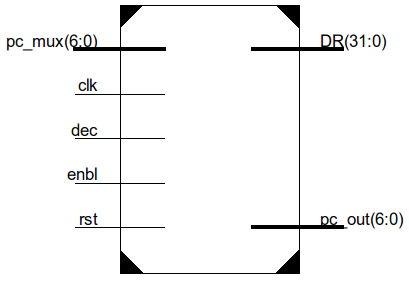
\includegraphics[scale=0.35]{Capitulo01/fetchstage}
\caption{Etapa de b\'usqueda}
\label{fig:fetch}
\end{figure}

\subsection{Funcionamiento}
El \texttt{pc} comienza de 0 y este valor entra en la memoria de instrucciones y en un m\'odulo sumador. En la memoria para que utilice la instrucci\'on ubicada en la posici\'on del mismo valor de contador de programa, y en la entrada del m\'odulo sumador se aumenta en 1 el valor para poder avanzar en el pr\'oximo ciclo de clock a una nueva instrucci\'on. Las salidas de esta etapa son la instrucci\'on a ejecutar y el valor del contador de programa.  (ver Figura \ref{fig:fetchzoom})

\begin{figure}[H]
\centering
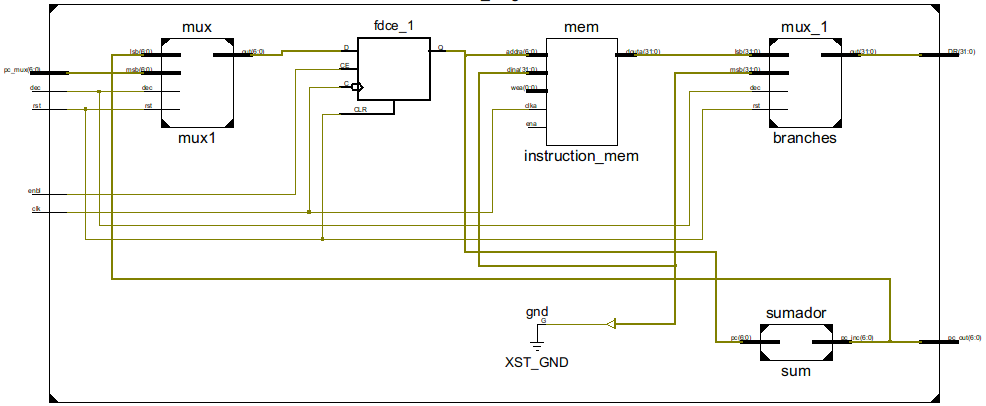
\includegraphics[scale=0.35]{Capitulo01/etapafetchzoom}
\caption{Etapa de b\'usqueda}
\label{fig:fetchzoom}
\end{figure}

\subsection{Multiplexor}

El m\'odulo multiplexor es binario, o sea que solamente elige entre dos valores. En nuestro caso debe escoger entre el \texttt{pc} que viene incrementado desde el m\'odulo sumador o el que viene modificado por un salto desde la etapa de ejecuci\'on. 

\begin{figure}[H]
\centering
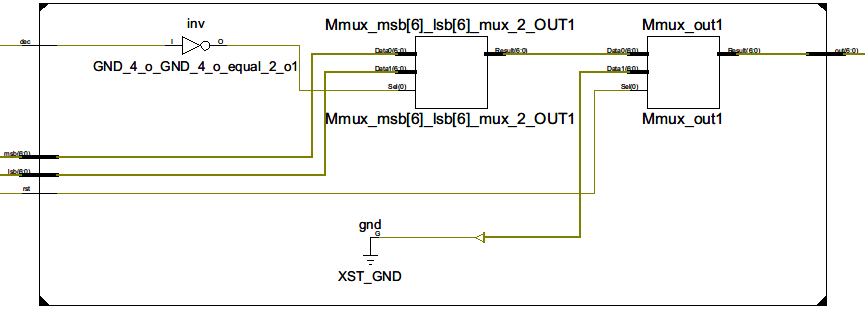
\includegraphics[scale=0.4]{Capitulo01/mux_fig.png}
\caption{M\'odulo multiplexor}
\label{fig:muxmodule}
\end{figure}

En la entrada del multiplexor entran 12 cables para que elija entre la parte alta y la parte baja, dependiendo de si es 1 o 0. Como lo programamos, cuando \texttt{dec} est\'a en uno elige el \texttt{pc}  que viene incrementado. En el otro caso, elige el que esta modificado por la etapa de ejecución.

\begin{figure}[H]
\centering
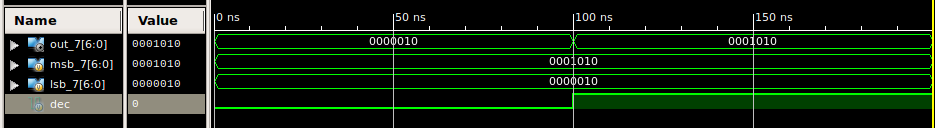
\includegraphics[scale=0.4]{Capitulo01/mux_test}
\caption{Testbench del multiplexor}
\label{fig:muxt}
\end{figure}

\subsection{Incremento}
El m\'odulo sumador simplemente incrementa el \texttt{pc}, tiene solamente una entrada que es un bus de 7 bits y este valor es incrementado dentro del m\'odulo. 


\begin{figure}[H]
\centering
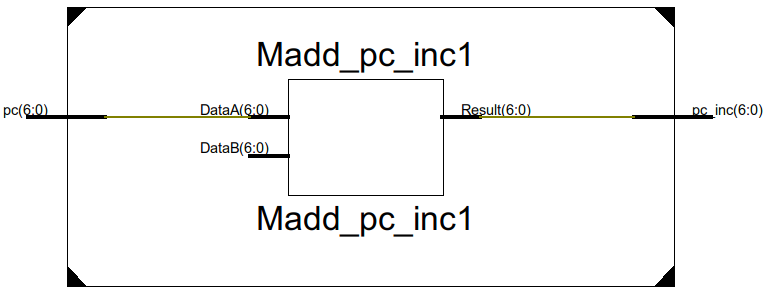
\includegraphics[scale=0.45]{img/sumador_inside}
\caption{Modulo sumador}
\label{fig:sumador}
\end{figure}


En el testbench contador de programa se va modificando de a uno, entonces la salida que en este caso es \texttt{pc\_inc} y esta ingresa en el registro del \texttt{PC}. 


\begin{figure}[H]
\centering
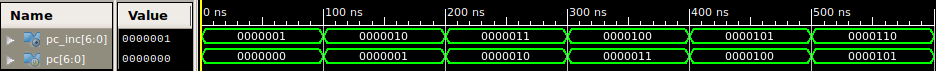
\includegraphics[scale=0.45]{Capitulo01/sum_test}
\caption{Testbench del sumador}
\label{fig:sumt}
\end{figure}


\subsection{Etapa de búsqueda con m\'odulos integrados}
Finalmente generamos un m\'odulo que integra los m\'odulos anteriores y terminamos la etapa. En este clock solamente el registro \texttt{pc} cambiaría de valor. 

\begin{figure}[H]
\centering
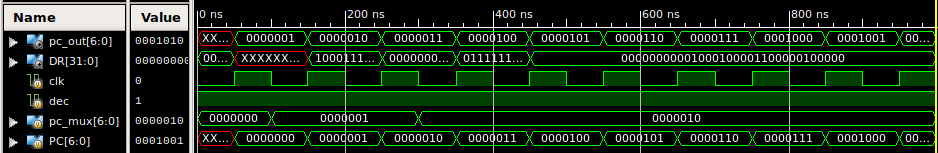
\includegraphics[scale=0.45]{Capitulo01/fetch_test}
\caption{Testbench del modulo fetch}
\label{fig:fetcht}
\end{figure}

Para entender que hace esta etapa podemos ver los cambios en la figura \ref{fig:fetcht}. Debemos comenzar viendo que \texttt{PC} no tiene ning\'un valor y es el que le ingresara en el clock a la memoria de instrucciones, \texttt{pc\_out} tampoco contiene ning\'un valor y este entra en el multiplexor (la memoria de instrucciones se puede ver en \ref{a.coe}).  
En el primer clock ascendente como \texttt{dec} esta en uno, elige \texttt{pc\_mux} para escribir al \texttt{pc} todos ceros, o sea, la primera direccion de memoria. El \texttt{dr}  muestra solo x porque en el clock anterior el \texttt{pc} estaba en x y en la memoria no direcciona en ninguna posici\'on valida. En el pr\'oximo clock ascendente ya el \texttt{pc} contiene ceros por lo que autom\'aticamente \texttt{pc\_out} va a tener el valor de \texttt{PC} + 1, pero \texttt{dec} esta en 1 por lo que sigue eligiendo a \texttt{pc\_mux}, que en el clock descendente anterior ya se le hab\'ia aumentado el valor en 1 por lo que este valor va a ser ingresado en el pr\'oximo clock al \texttt{pc} y \texttt{dr} ya comienza a mostrar el primer valor de la memoria de instrucciones. Los siguientes clocks funcionan de la misma manera.

\lstinputlisting[label=a.coe, caption=Contenido de la memoria de instrucciones, captionpos=b]{Capitulo01/a.coe}	
	\appendix
\chapter{Etapa de búsqueda}
\lstinputlisting[label=mux, caption=Modulo multiplexor, captionpos=b]{apendice/fetch/mux_7bit.v}
\lstinputlisting[label=mux_test, caption=Test del modulo multiplexor, captionpos=b]{apendice/fetch/mux_test.v}
\lstinputlisting[label=sum, caption=Modulo sumador, captionpos=b]{apendice/fetch/sumador.v}
\lstinputlisting[label=sum_test, caption=Test del modulo sumador, captionpos=b]{apendice/fetch/sumador_test.v}
\lstinputlisting[label=fetch, caption=Modulo fetch, captionpos=b]{apendice/fetch/fetch_stage.v}
\lstinputlisting[label=fetch_test, caption=Test del modulo fetch, captionpos=b]{apendice/fetch/fetch_test.v}
%--------------------------------------------------------
% Apendice
%--------------------------------------------------------
	%\input{}

%--------------------------------------------------------
% Bibliografia
%--------------------------------------------------------
	\begin{thebibliography}{9}
 		 \bibitem{bib:Coad} Computer Organization and design - David A. Paterson, John L. Hennessy
 		 %\cite{ref} para referenciar en el texto
	\end{thebibliography}
	
	\section*{Lista de Acrónimos}\medskip
	\begin{acronym}[SIGCOMM]
		\acro{pc}[PC] {contador de programa}
		\acro{dr}[DR] {registro de datos}
	\end{acronym}
	
%--------------------------------------------------------
% Fin del documento
%--------------------------------------------------------

\end{document}